\documentclass{beamer}


% Load essential packages
\usepackage{hyperref} % Only load once to avoid conflicts
\usepackage{stile}
\usepackage{subcaption}
\usepackage{tcolorbox}
\usepackage[font=scriptsize,skip=1pt]{caption}
\usepackage[T1]{fontenc}
\usepackage{csquotes}
\usepackage[backend=biber, style=authoryear, maxnames=3, minnames=1, abbreviate=false, date=long, url=false, isbn=false, doi=false]{biblatex}
\addbibresource{lecture7/bib.bib} % Ensure this matches your bibliography file name

\interfootnotelinepenalty=10000

\usepackage{latexsym, amsmath, xcolor, multicol, booktabs, calligra}
\usepackage{graphicx, pstricks, listings, stackengine}

% Hyperref setup
\hypersetup{
    hidelinks,
    colorlinks=true,
    linkcolor=black,
    citecolor=blue,
    urlcolor=black
}

% Font theme for Beamer
\usefonttheme[onlymath]{serif}

% Custom definitions
\def\cmd#1{\texttt{\color{red}\footnotesize $\backslash$#1}}
\def\env#1{\texttt{\color{blue}\footnotesize #1}}
\definecolor{deepblue}{rgb}{0,0,0.5}
\definecolor{deepred}{rgb}{0.6,0,0}
\definecolor{deepgreen}{rgb}{0,0.5,0}
\definecolor{halfgray}{gray}{0.55}

% Beamer color settings
\setbeamercolor{block title}{bg=blue!70!white, fg=white}
\setbeamercolor{block body}{bg=blue!10!halfgray, fg=white}
\setbeamercolor{section in head/foot}{fg=white}
\setbeamercolor{subsection in head/foot}{fg=white}
\setbeamercolor{title in head/foot}{fg=white}


% Listings settings for code highlighting
\lstset{
    basicstyle=\ttfamily\small,
    keywordstyle=\bfseries\color{deepblue},
    emphstyle=\ttfamily\color{deepred},
    stringstyle=\color{deepgreen},
    numbers=left,
    numberstyle=\small\color{halfgray},
    rulesepcolor=\color{red!20!green!20!blue!20},
    frame=shadowbox,
}

% Title page info
\author{Freya Rubel}
\title{Trade, Migration and Global Challenges}
\subtitle{Migration and Global Welfare}
\institute{}
\date{11.12.2025}

\graphicspath{{lecture7/}}

\begin{document}

\begin{frame}
    \titlepage
\end{frame}

\begin{frame}{Announcement: Exam Date confirmed}
\centering
\vspace{0.5cm}

\begin{tcolorbox}[colback=red!5!white,colframe=red!75!black,title=Final Exam]
\centering
\Large
\textbf{Date:} 19.02.2026 at 10:15am \\
\textbf{Room:} 201 \\
\end{tcolorbox}

\vspace{0.5cm}
\begin{normalsize}
Please arrive at 10:00am! The exam is scheduled for 90 minutes. Bring your student ID.
\end{normalsize}

\end{frame}

\begin{frame}
    \tableofcontents[sectionstyle=show, subsectionstyle=show/shaded/hide, subsubsectionstyle=show/shaded/hide]
\end{frame}

\section{Recap - Welfare}
\begin{frame}{Economic Definition of Welfare}
    Welfare refers to the cumulative well-being/standard of living/utility/happiness of individuals (and groups) within an economy. 
    \begin{itemize} \small
        \item \textbf{Material Well-Being:} Access to income, goods, and services that allow individuals to consume food, shelter, clothing, etc. 
        \item \textbf{Non-Material Well-Being:} Factors such as health, education, safety, leisure, social connections, and environmental quality, which contribute to a higher quality of life.
        \item \textbf{Economic Security:} Prospect of stability in employment and income, safety nets to protect against economic shocks. Institutions, systems, and an environment that allows for sustained material well-being.
        \item \textbf{Freedom of Choice:} The ability to make (economic) decisions freely, reflecting individual preferences.
    \end{itemize}
\end{frame}

\begin{frame}{Individual Utility Functions}
Utility represents the satisfaction/benefit that an individual receives from consuming goods or services. Individual utility is defined as a function of the consumption of goods and services, such as food, clothing, and the natural environment. \\
\textbf{Utility is an ordinal concept:} \pause The values of utility assigned to the consumption of certain bundles of consumption determine which bundle of consumption gives you a higher welfare but you cannot compare by how much.
$$U(x_1, x_2, x_3, L) = \alpha ln(x_1) + \beta ln(x_2) + \gamma ln(x_3)  + \delta L $$ % does anyone know why we typically take the logarithm of the quantity of goods and ervices in a utility function?
$$\text{Example: } U(2,4,4,8)>U(1,2,2,4) \text{ but } U(2,4,4,8) \neq 2\times U(1,2,2,4)$$
\end{frame}

\begin{frame}{Reminder: Indifference Curves}
    \begin{figure}
        \centering
        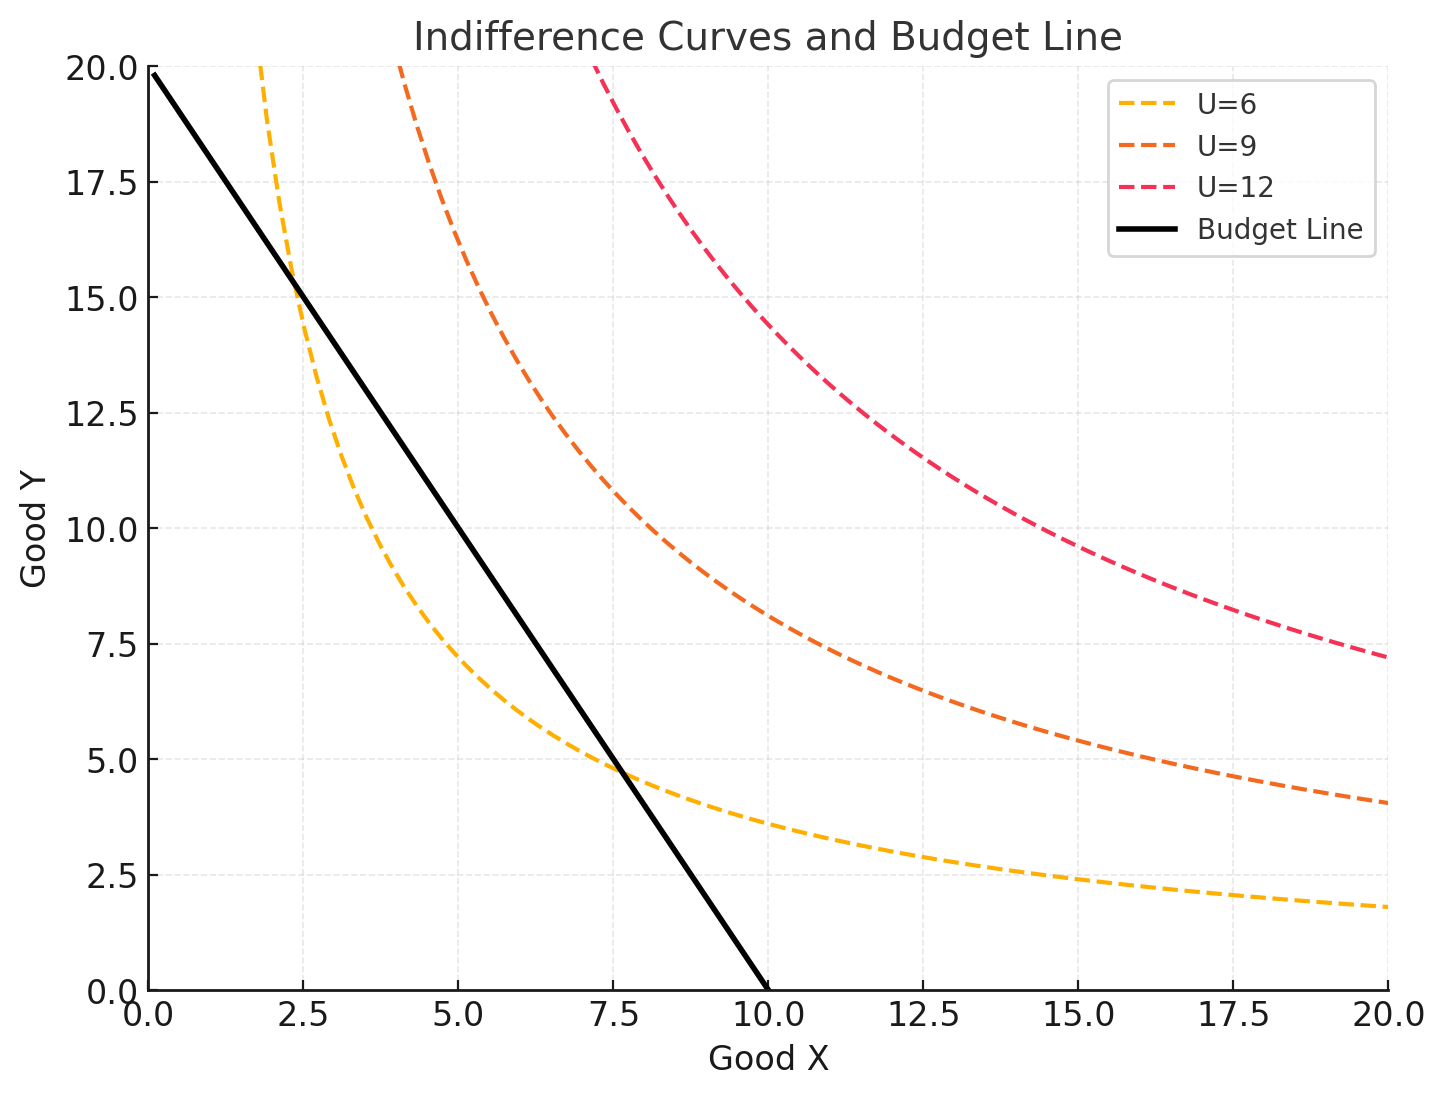
\includegraphics[width=0.8\linewidth]{indifference_curves and budget.png}
        \label{fig:enter-label}
    \end{figure}
\end{frame}

\begin{frame}{Social Welfare Function}
    A social welfare function is a function that ranks a set of states by their desirability. Each individual's preferences are aggregated \textbf{in some way} to determine which outcome is preferred by society as a whole. 
     $$W=F(U_1, U_2, U_3, ..., U_n)$$
    If we aggregate by summing the utility of each individual ($W = \sum_{i=1}^{n} U_i$) and choose the state that maximizes this sum, this is \textit{utilitarianism}.
\end{frame}

\begin{frame}{Reminder: Welfare Gain from Migration}
    \begin{figure}
        \centering
        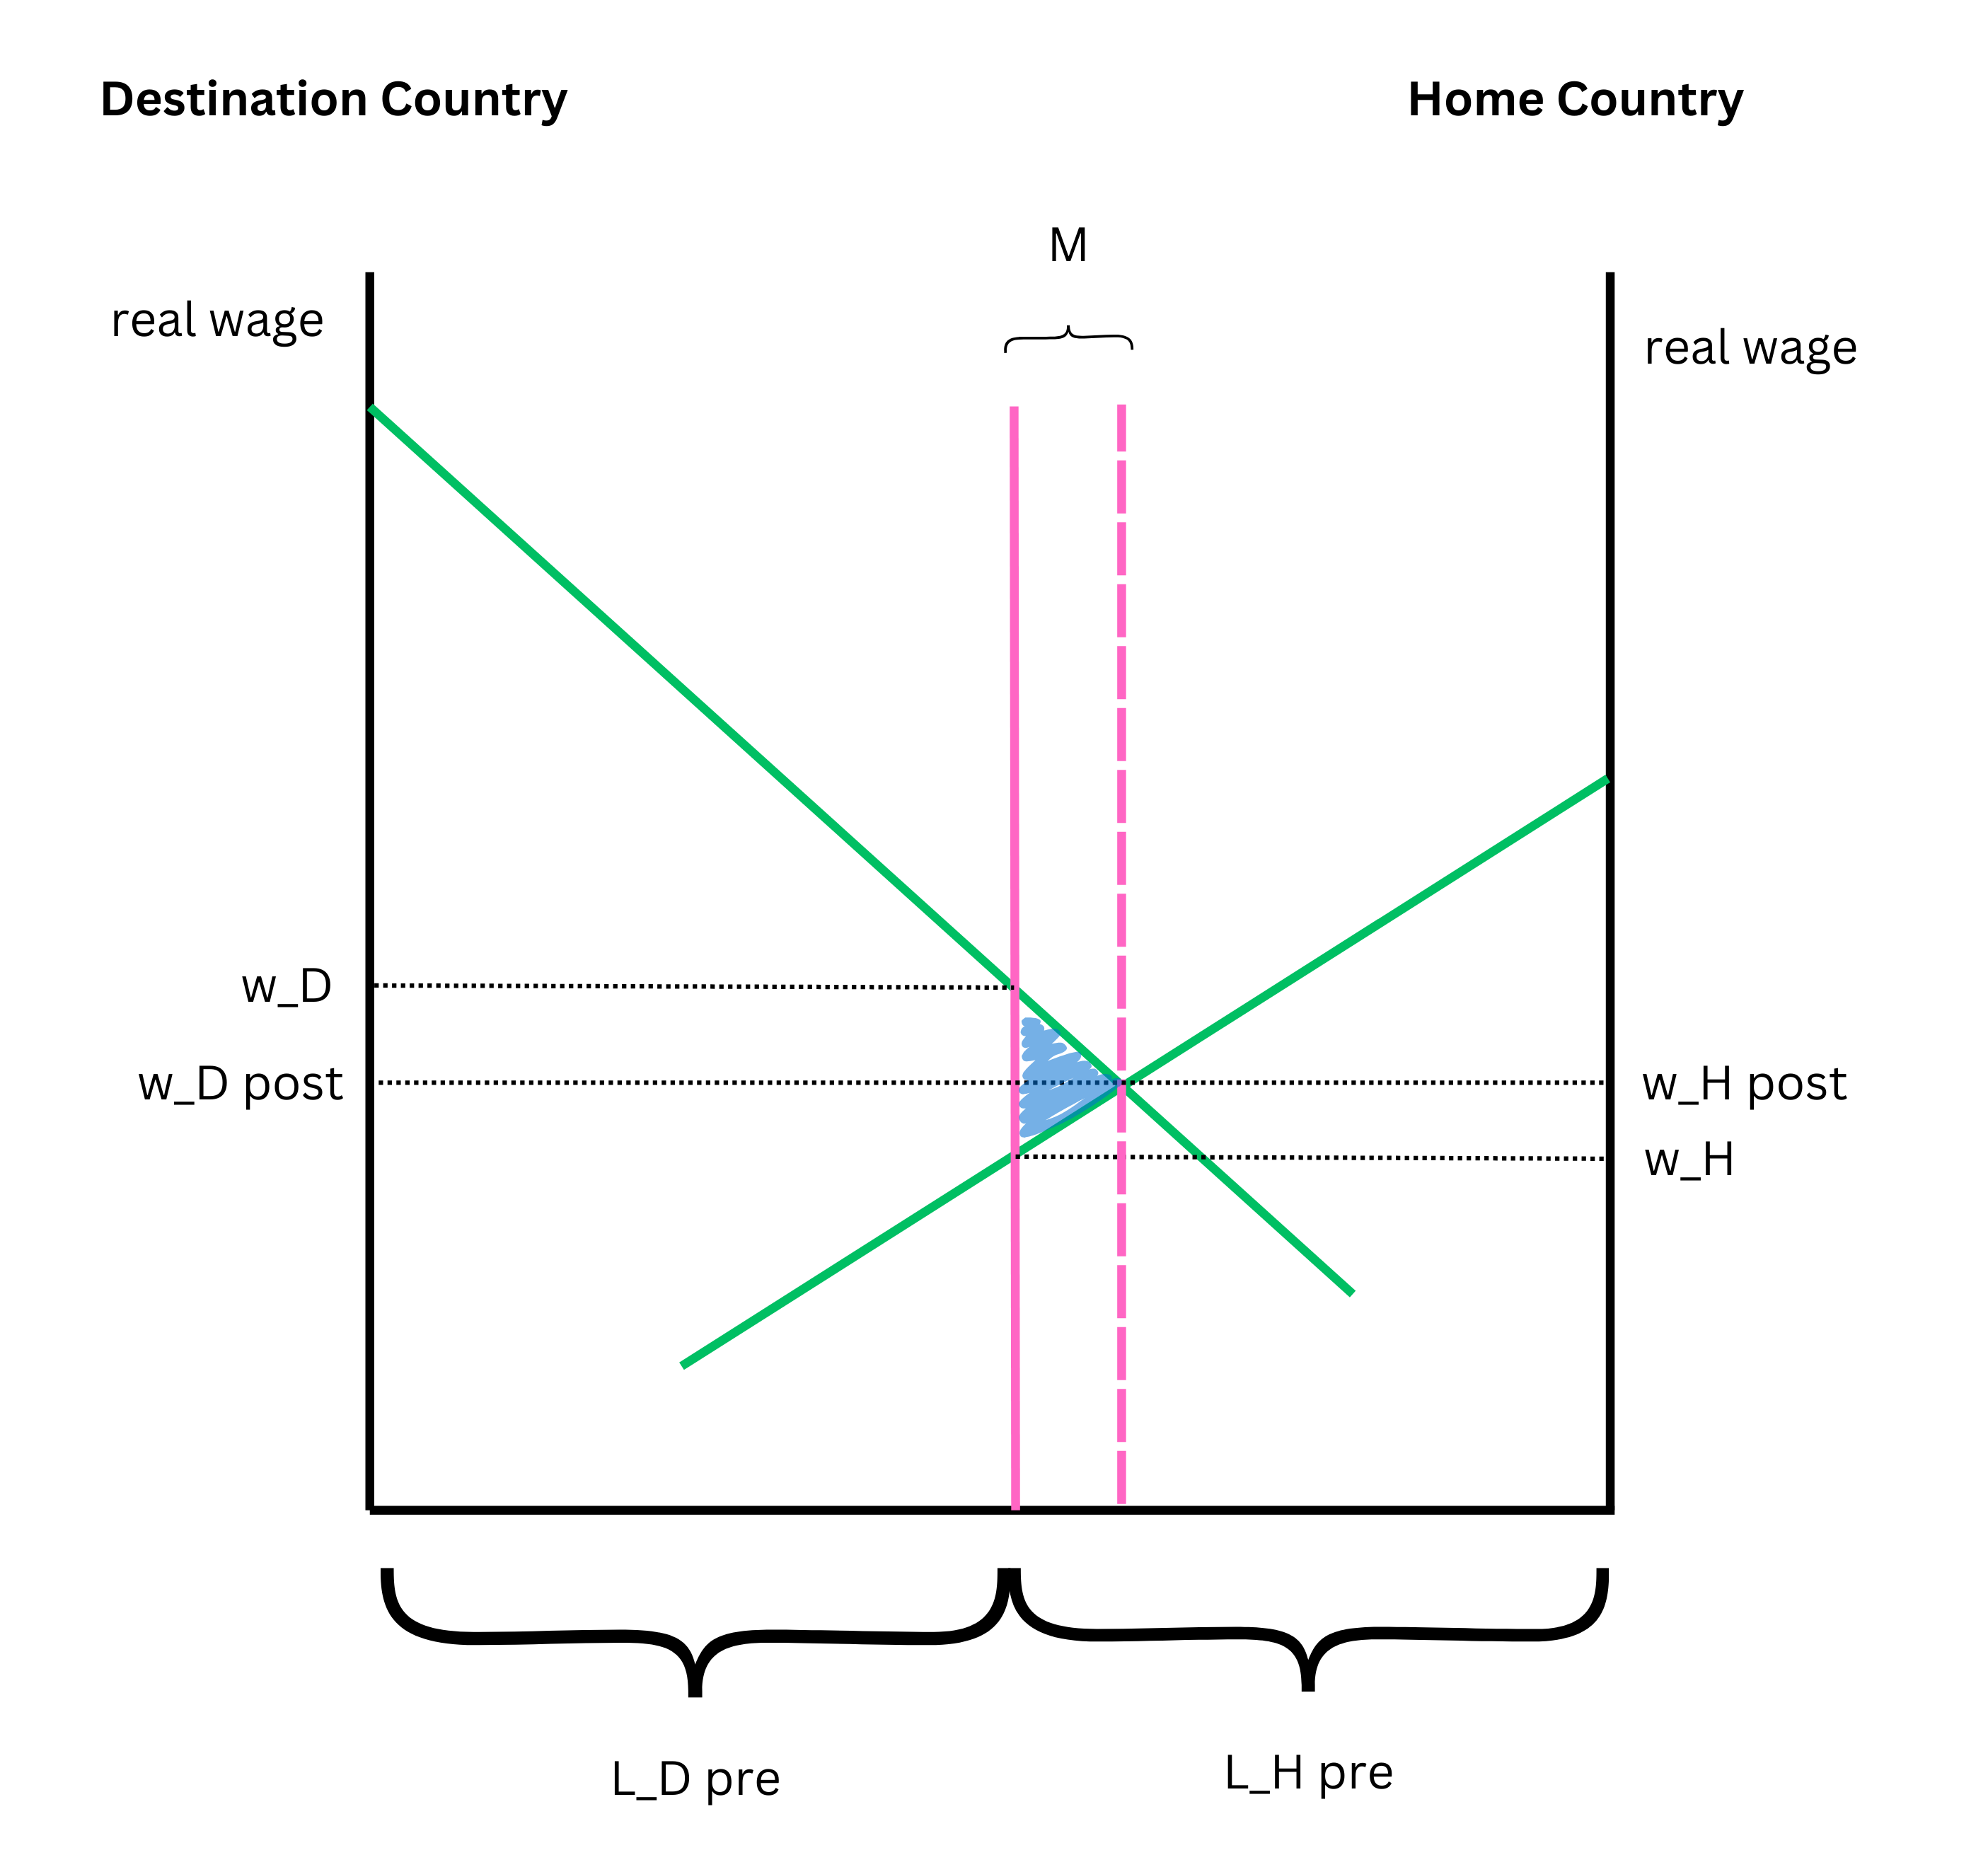
\includegraphics[width=0.7\linewidth]{wage equalization with free movement.png}
        \label{fig:enter-label}
    \end{figure}
\end{frame}

\begin{frame}{Interpretation of the Welfare Gain}
    \begin{itemize} \small
        \item Free international migration contributes to global efficiency (there is a “global welfare gain”).
        \item The loss in economic welfare in the sending country is more than compensated by an increase in welfare in the receiving country. 
        \end{itemize}
        \textbf{However...}
    \begin{itemize} \small
        \item Externalities in host countries: threats to social cohesion, effects on inequality, ...
        \item Externalities in home countries: brain drain, effects on inequality (through selection and remittances), ... % apart from that, in order to have that kind of gains from migration, you don't simply need open borders, you need proper integration into the receiving labor market as well 
    \end{itemize}
\end{frame}

\begin{frame}{Shortcomings of our common indicator of welfare: income}
\textbf{Example:} \\
Imagine a worker with above average income in a poor country migrates to a rich country and now makes twice as much in real wages. However, this wage is below the average wage in the destination country. Let's suppose that there is no effects on anyone else. \\
What happens to average income in the \textit{sending} location? \pause It falls. \\ \pause
What happens to average income in the \textit{receiving} location? \pause It falls. \\
Is migration decreasing overall welfare? \\ \pause % no, if noone was affected and this person is now earning more than before, we should aggregate 
Alternative measurement: Focus on average income per \textit{natural} - the income of people born in a certain place.
\end{frame}

\section{Trade}
\begin{frame}{The Trade-Creating Effect of Migration}
International migration creates international trade. Why? \pause 
\begin{itemize} \small
    \item Information effect: Migrants reduce bilateral information costs. % migrants facilitate information flow on foreign markets. They provide information about a place where the business might want to expand to
    \item Preference effect: Migrants increase demand for products from their home country in their host country. % supermarkets
    \item Network Effect: Migrants create and strengthen trade networks, facilitating partnerships and reducing transaction costs between their home and host countries. % migrants still have ties to their region of origin, possibly former employers that were working in the same industry. These relationships are very strong in predicting, which partners you are trading with in the future. If you can choose out of a number of international businesses, you might choose the business that you have personal contact with and that is from your own nationality
    \item Innovation Effect: Migrants introduce new ideas, products, and services that can create new markets and expand trade opportunities. % I gave you the example of danish migrants that considerably drove innovation in the dairy industry in the US. YOu have the same effect from hugenots migrating to Prussia in the 17th century that advanced textile production. 
\end{itemize}
\end{frame}

% Slide 1
\begin{frame}{Paper Presentation}
\centering
\begin{Large}
    Migrant Networks and Trade: \\ The Vietnamese Boat People as a Natural Experiment \\
\end{Large}
\begin{large}
    Christopher Parsons and Pierre-Louis Vézina \\
\end{large}
Published in The Economic Journal (2018)
\end{frame}

% Slide 2
\begin{frame}{Research Motivation}
\textbf{Theory and Background}
    \begin{itemize}
        \item Migrants facilitate international trade by reducing trade costs and creating demand.
        \item Existing literature shows a correlation between migration and trade, but causality is not clearly established.
        \item \textcite{ParsonsChristopher2018MNAT} exploit a natural experiment: The migration of \textit{Vietnamese Boat People} to the U.S. after the Fall of Saigon.
        \item Between 1975 and 1994, around 1.4 million Vietnamese refugees settled in the U.S.
    \end{itemize}
\end{frame}

% Slide 3
\begin{frame}{Research Question}
    \begin{itemize}
        \item \textbf{Main Question:} Did the Vietnamese population in the U.S. create long-term economic benefits by fostering trade between the two countries?
        \item \textbf{Specific Focus:} How did the resettlement of Vietnamese refugees in the U.S. influence trade with Vietnam after the lifting of the trade embargo in 1994?
    \end{itemize}
\end{frame}

% Slide 4
\begin{frame}{Methodology}
\textbf{Natural Experiment:}
        \begin{itemize}
            \item Quasi-random dispersion of Vietnamese refugees across U.S. states in 1975 due to resettlement policies and urgency of the situation. % in these type of displacement of people, we are on the side of forced migration and this doesn't take place orderly by evaluating which regions might be very wlecome to migrants or offer the highest economic potential
            \item Trade embargo until 1994 $\rightarrow$ definitely no reverse causality between migration and trade.
        \item \textbf{Instrumental Variable:} Refugee distribution in 1975 predicts Vietnamese population in 1995, which is the variable of interest.% there were several waves after 1975 but we believe the random allocation in 1975 to predict a relevant share of the variation that we do see in the population in 1995.
        \item \textbf{Outcome Variable}: trade between the U.S. and Vietnam between 1995 and 2010.
    \end{itemize}
\end{frame}

% Slide 5
\begin{frame}{Data}
    \begin{itemize}
        \item \textbf{Migration Data:} Refugee allocations from the U.S. General Accounting Office (1975), Vietnamese population from the 2000 U.S. Census.
        \item \textbf{Trade Data:} U.S. exports to Vietnam (1995–2010) categorized by product type from UN Comtrade.
        \item \textbf{Control Variables:} State GDP, income per capita, manufacturing share, and coastal proximity.
    \end{itemize}
\end{frame}

% Slide 6
\begin{frame}{Key Findings}
    \begin{itemize}
        \item A 10\% increase in Vietnamese migrants in a U.S. state led to a 4.5–14\% increase in exports from that state to Vietnam.
       \item Effect concentrated in \textbf{differentiated goods} where information matters most (no effect for homogeneous goods).
        \item Counterfactual analysis: exports would have been approximately 50\% lower without the Vietnamese migrants in the top 10 states.
    \end{itemize}
\end{frame}

% Slide 8
\begin{frame}{Mechanisms}
\begin{itemize}
    \item Placebo tests showed Vietnamese migrants had no effect on US exports to 10 other Asian countries $\rightarrow$ serves as evidence against a "change in racial attitudes" mechanism.
\end{itemize}
Most probable channels proposed by the authors:
    \begin{itemize}
        \item \textbf{Information Channel:} Vietnamese migrants reduced information barriers (language, market knowledge, business practices) helping US firms export to Vietnam.
        \item \textbf{Network/Trust Channel:} Vietnamese migrants facilitate contract enforcement and reduce opportunistic behavior through trusted networks in weak institutional environments.
    \end{itemize}
\end{frame}

% Slide 9
\begin{frame}{Policy Implications}
    \begin{itemize}
        \item \textbf{For Host Countries:} Migrants are an asset, able to enhance trade ties and economic growth for the receiving region.
        \item \textbf{For Origin Countries:} Engaging the diaspora through incentives can foster development through greater market integration. \textcolor{red}{But mind a brain drain or the creation of dependencies.}
        \item Suggests broader gains from migration liberalisation, which are usually not considered in political debates about migration.
    \end{itemize}
\end{frame}

\section{Financial Flows}
\begin{frame}{Foreign Direct Investment (FDI)}
    \textbf{Migration can reduce risk and uncertainty.} Hypothesis: migration should stimulate bilateral financial flows thanks to information from migrants to investors.
    \begin{itemize} \small
        \item Facilitate the formation of business links.
        \item Catalyst to establish efficient distribution, procurement, and transportation.
        \item \textcite{FoleyC.Fritz2013EIaU} show that firms with more patenting activity performed by inventors from a certain ethnicity have higher FDIs to the inventors’ countries of origin.

    \end{itemize}
\end{frame}

\begin{frame}{Foreign Financial Flows to LMIC}
    \begin{figure}
        \centering
        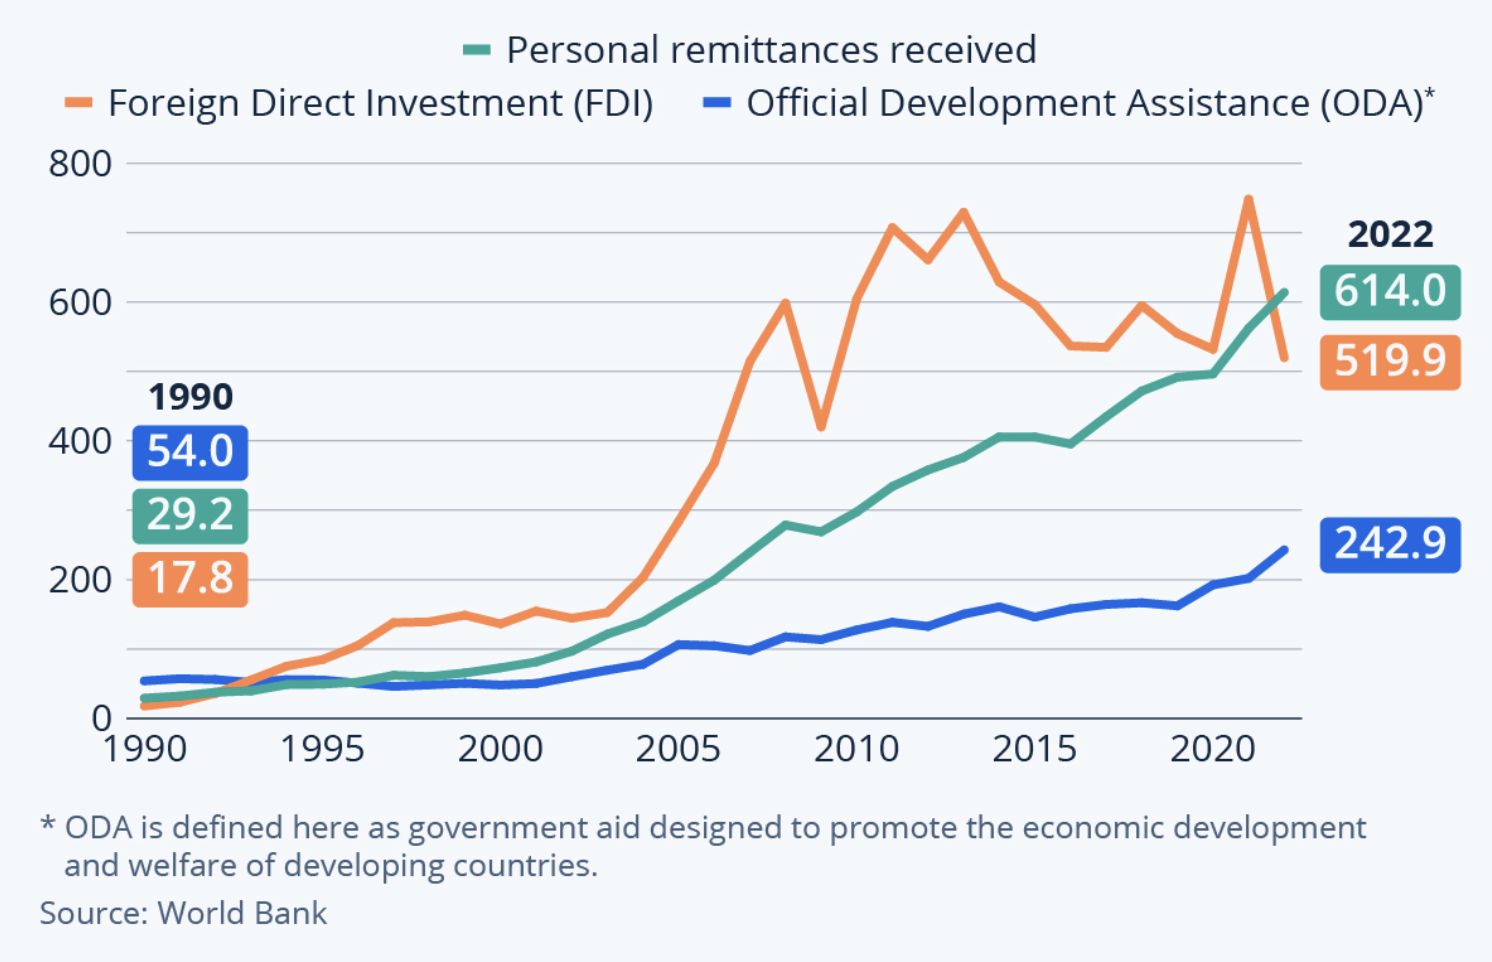
\includegraphics[width=\linewidth]{FDI, remittance and ODI.png}
        \caption{Received by low- and middle-income countries}
        \label{fig:enter-label}
    \end{figure}
\end{frame}

\begin{frame}{Top Destinations of Remittances}
    \begin{figure}
        \centering
        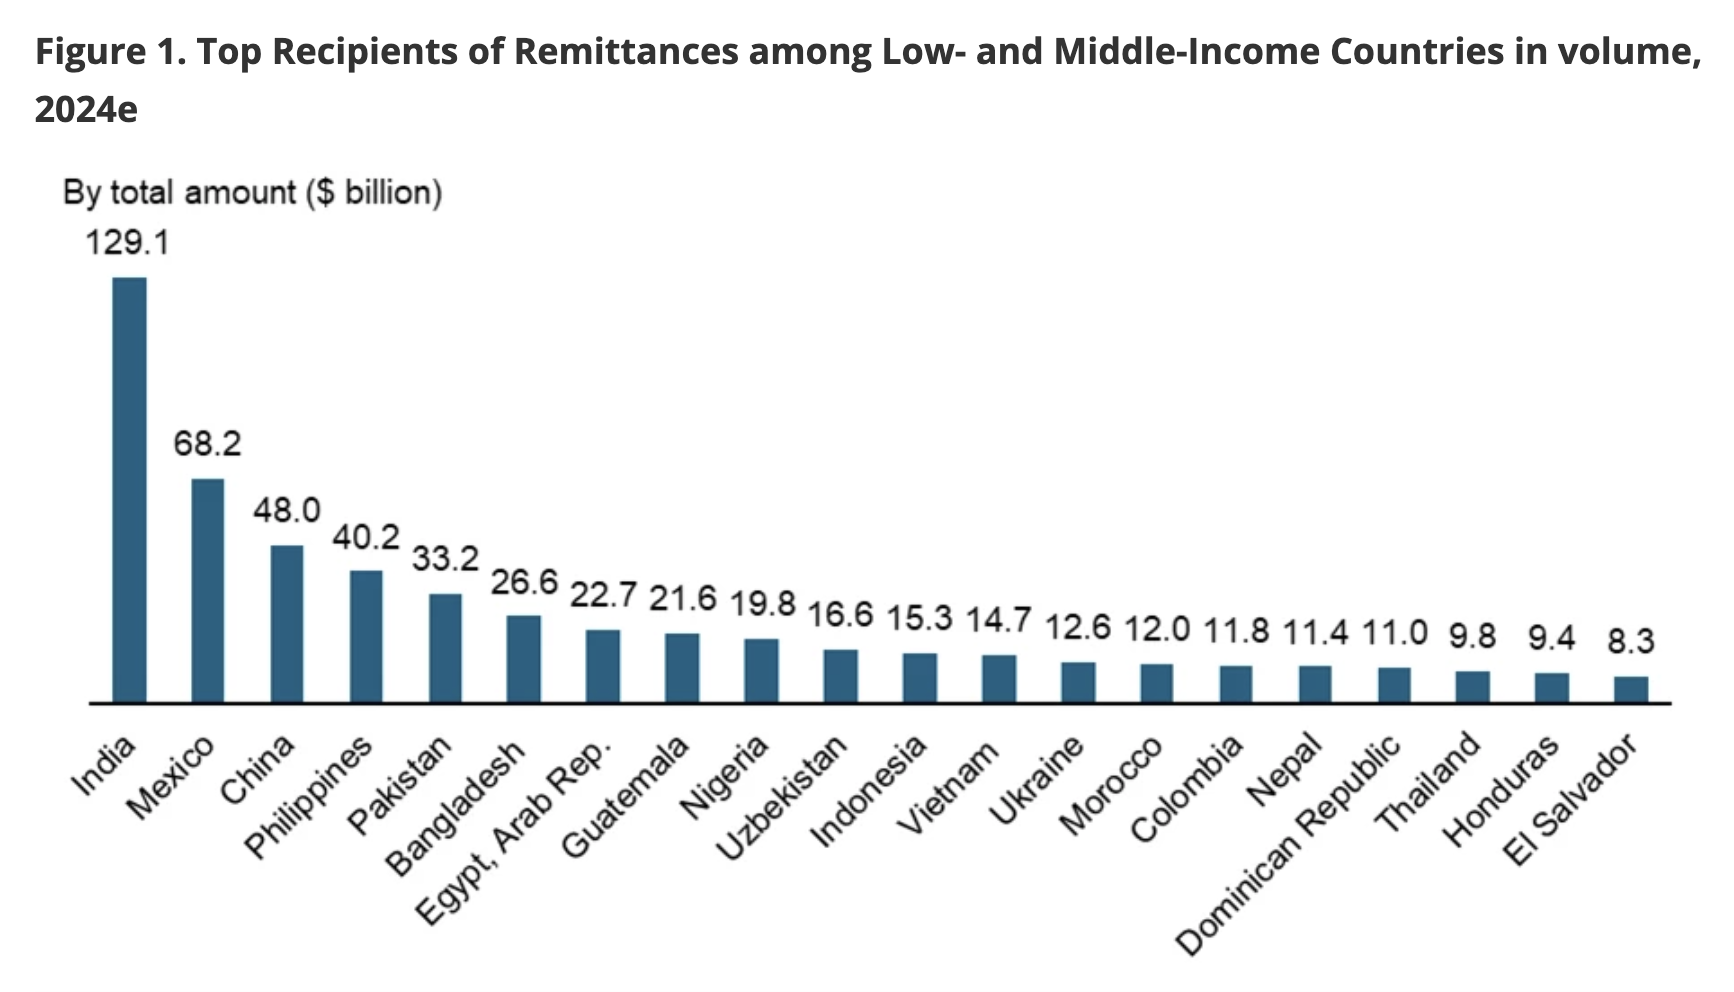
\includegraphics[width=\linewidth]{recipientsremittances.png}
        \label{fig:enter-label}
    \end{figure}
\end{frame}

\begin{frame}{Share of Remittances in total GDP}
    \begin{figure}
        \centering
        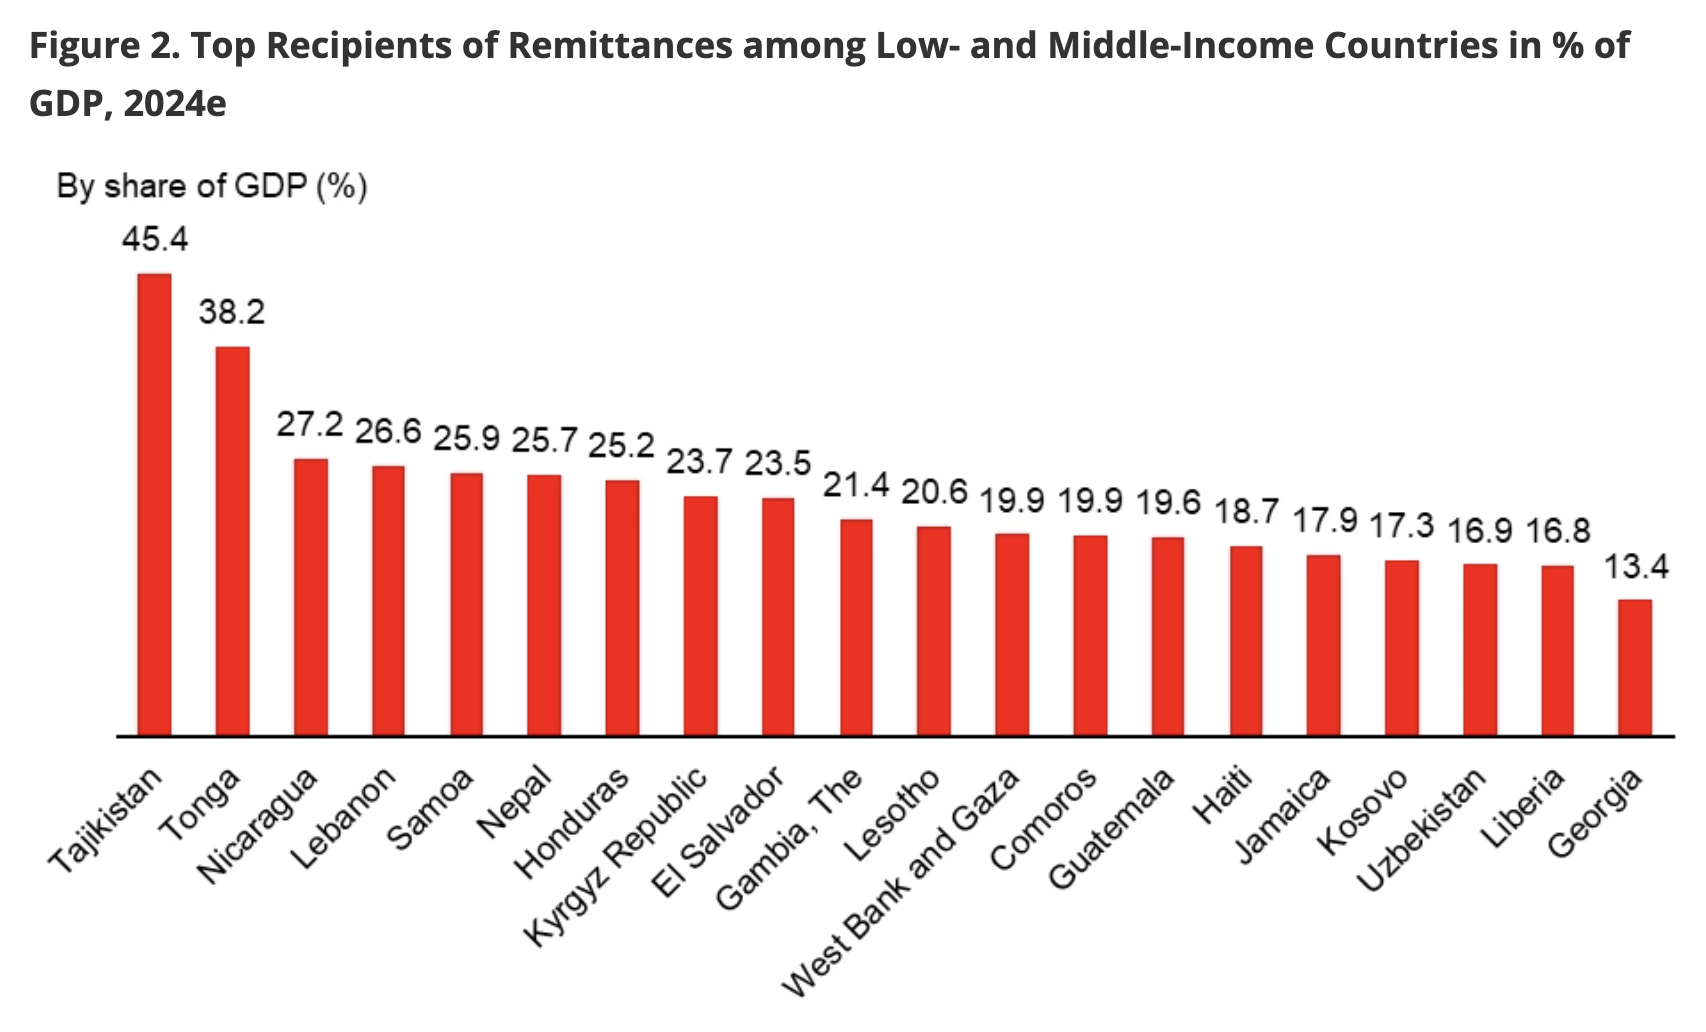
\includegraphics[width=\linewidth]{share_remittances.png}
        \label{fig:enter-label}
    \end{figure}
\end{frame}

\begin{frame}{Remittances: Beyond Financial Flows}
    Remittances are more stable than other capital flows and have distinct welfare effects:
    \begin{itemize}
        \item \textbf{Consumption smoothing}: Counter-cyclical during economic downturns in origin countries
        \item \textbf{Financing human capital investment}: Households typically use remittances to increase spending on education and health
        \item \textbf{Entrepreneurship}: Funding for small business creation
        \item \textbf{Potential costs}: Moral hazard (reduced labor supply), Dutch disease effects if large relative to GDP % have you heard the term dutch disease before? It means that large flows of money into the economy are strengthening a country's currency, which makes the tradeble sector like manufacturing less competitive. When the currency is strengthened, the exchange rate makes foreign products seem cheaper and domestic production appears more expensive to consumers abroad, which makes your imports grow and your exports shrink. Lower net exports are decreasing your GDP 
    \end{itemize}
\end{frame}

\section{Technology Diffusion}
\begin{frame}{Technological Spillover}
    \begin{itemize}
        \item Knowledge diffusion tends to be highly geographically localised.
\item \textbf{Tacit knowledge} refers to skills, expertise, or know-how that are difficult to codify or communicate in written or verbal forms. It is often best learned through direct experience or interaction.
\item Thus, the pattern of international knowledge diffusion should relate to the pattern of international migration: immigrants “bring” knowledge; emigrants can transfer knowledge back home.
    \end{itemize}
\end{frame}

\begin{frame}{Technology Diffusion: Empirical Evidence}
    \begin{itemize}
        \item \textcite{Fackler2020KnR} find that emigration positively contributes to innovation in source countries (32 European countries).
       \item \textcite{Kerr2008EtaI} confirm by use of international patent citations that knowledge diffuses through ethnic networks.
       \item Doubling the number of migrant inventors from countries that specialise in a technology increases the probability of gaining technological advantage in that technology by 25-60\% (\cite{Bahar2020MIT})
    \end{itemize}
\end{frame}

\begin{frame}{Technology Transfer Through Return Migration}
    Return migrants bring accumulated human capital back to origin countries:
    \begin{itemize}
        \item \textbf{Embodied knowledge}: Skills and expertise acquired abroad
        \item \textbf{Network effects}: Maintained connections facilitate ongoing knowledge transfer
        \item \textbf{Entrepreneurship}: Return migrants more likely to start businesses 
        \item Example: Return migration to India and China with Silicon Valley connections contributed to tech sector growth in their home country.
    \end{itemize}
\end{frame}


\begin{frame}[allowframebreaks]{References}
    \printbibliography
\end{frame}


\end{document}

